\subsection{Vue d'ensemble de \nameTool}\label{sec:sat_interface}


\nameTool\ est composé de trois modules, mais l'utilisateur standard ne verra que l'un d'entre eux : l'interface. Dans la suite nous insistons principalement sur cette dernière plut\^ot que sur le traducteur et le solveur. L'architecture globale est illustr\'{e}e par la figure~\ref{fig:architectureTouisT}: 

\begin{figure}[htbp]
\centering
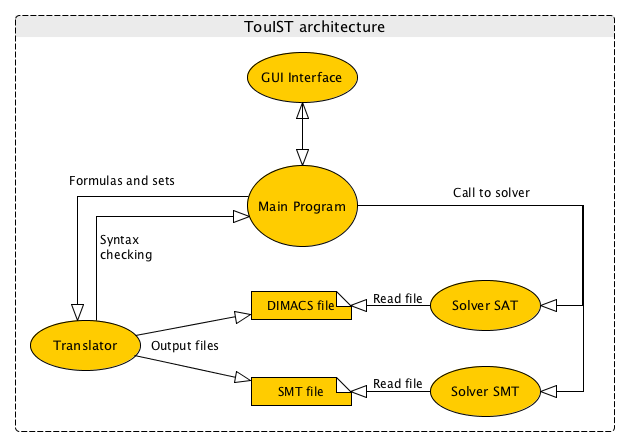
\includegraphics[scale=0.37]{Pictures/DiagTouist.png}
  \caption{Architecture de TouIST}
  \label{fig:architectureTouisT}
\end{figure}

Avec \nameTool\ , on accède à un éditeur puissant et convivial pour éditer des formules logiques complexes et des contraintes variées comme :

$$\bigwedge_{i \in \{1..9\}} (P_i \IMPL Q_{i+1})$$

qui abrège confortablement :\\ 

$(P_1 \Rightarrow Q_2) \AND (P_2 \IMPL Q_3) \AND \ldots (P_9\IMPL Q_{10})$. 
\\

Une fois qu'un ensemble de formules a été donné à l'interface, sa satisfiabilité peut \^etre vérifiée : l'interface peut l'envoyer au prouveur qui retourne un modèle, affich\'{e} comme le montre la figure \ref{fig:ExampleOfAModel} si un tel mod\`{e}le existe. Ensuite par l'intermédiaire de l'interface, l'utilisateur peut par exemple demander d'autres modèles (bouton ``Next'' de l'interface). Contrairement à \satoulouse\ qui aurait nécessité de modifier les formules pour interdire le modèle et de relancer le solveur, \nameTool\ conserve une instance du solveur en attente, ce qui permet d'obtenir les modèles suivants bien plus rapidement.

\begin{figure}[htbp]
\centering
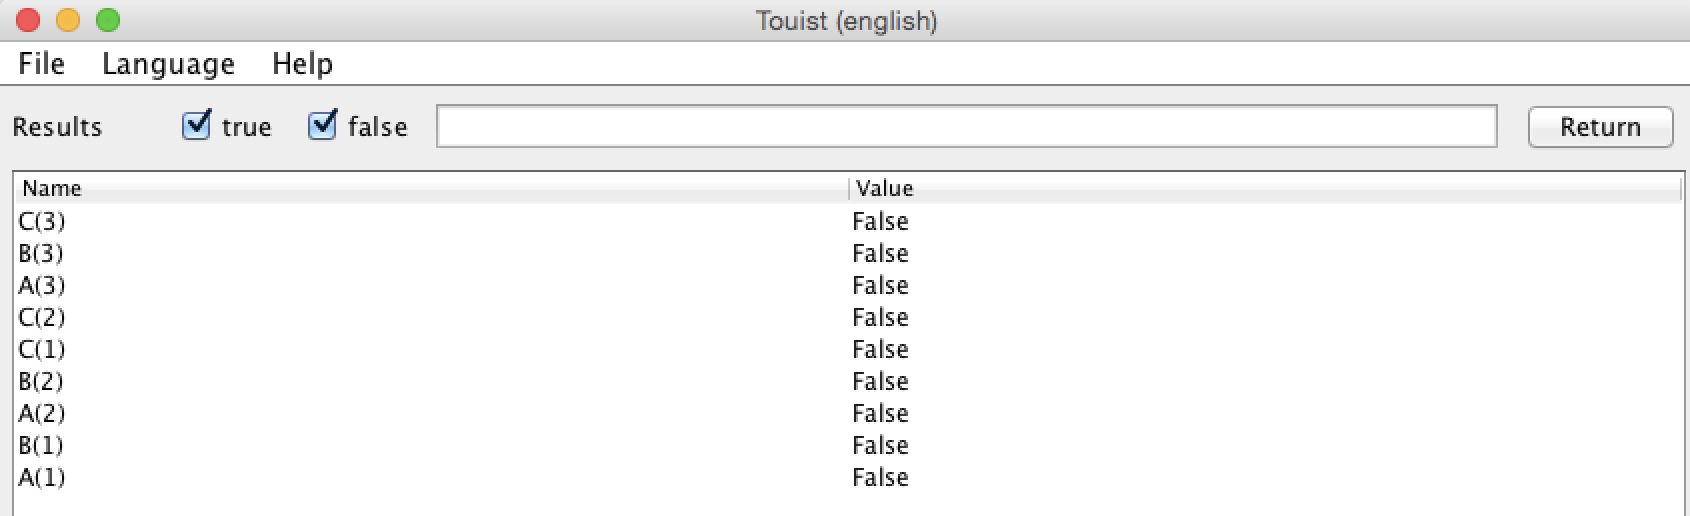
\includegraphics[scale=0.27]{Pictures/ExampleOfAModel.png}
  \caption{Affichage de mod\`{e}le}
  \label{fig:ExampleOfAModel}
\end{figure}

Les mod\`{e}les renvoy\'{e}s par le solveur sont totaux : une valeur est affect\'{e}e \`{a} chacune des variables apparaissant dans les formules envoy\'{e}es au solveur. L'utilisateur peut s\'{e}lectionner uniquement les propositions vraies ou les propositions fausses. Il peut \'{e}galement s\'{e}lectionner des sous-ensembles de variables en tapant une expression r\'{e}guli\`{e}re pour les filtrer.
